\section{Statistical Analysis of Experiment \#1}\label{sec:Stat1}

In this section, the various statistical methods covered in \cref{subsec:distribution} and \cref{subsec:correlation} will be used to analyze the data collected from experiment \#1. This analysis will first of all aim to check if the data is normally distributed as it has an effect on which statistical methods can be used in the later stages of the analysis. When checking if the data is normally distributed, the Shapiro-Wilk test\cite{razali2011power} will be used. In the next step of the analysis, the Mann-Whitney U Test\cite{mann1947test} will test if the different test case measurements are from the same population or not, and finally, the correlation between the different test case measurements will be calculated and analyzed.

\subsection{Normal Distribution}\label{subsec:NormalDist1}
The Shapiro-Wilk test will be used to test if the data is normally distributed, this is important as it affects which statistical methods can be applied to the test case measurements correctly when finding correlations as covered in \cref{subsec:distribution}. 

\paragraph{Expectations:} For the Shapiro-Wilk test the expectation is that the majority of the test case measurements will be normally distributed. This assumption is primarily based on the findings by Koedijk et al.\cite{Koedijk2022diff}. We expect most of the data to either be normally distributed, with some exceptions that behave differently.

\paragraph{Result:} The results for this experiment can be seen in \cref{tab:NormDistSurfB}. The values in this table are normally distributed if they are smaller than $p$, where $p = 0.05$\cite{wasserstein2019moving}. Based on this, most data can be concluded to be normally distributed, with a few exceptions like E3 on TestCaseIdle. Because not all data is normally distributed, the statistical methods able to handle data which is not normally distributed data are used. This is in line with what we expected based on the literature.

\begin{table}[]
    \begin{tabular}{||c|c|c|c|c|c||}
    \hline
    &\textbf{TestCaseIdle}&\textbf{BinaryTrees}&\textbf{FannkuchRedux}&\textbf{Nbody}&\textbf{Fasta}\\ [0.5ex] \hline\hline
    \textbf{IntelPowerGadget}&0.0004&0.3685&0.0007&0.0&0.0809\\
    \textbf{HardwareMonitor}&0.0&0.0033&0.088&0.0&0.0002\\
    \textbf{E3}&0.9307&0.2229&0.0&0.0966&0.0002\\
    \textbf{RAPL}&0.0152&0.0311&0.0&0.0&0.0007\\ \hline
    \end{tabular}
    \label{tab:NormDistSurfB}
\end{table}

\subsection{Independence Test}\label{subsec:independence1}

When testing the independence of data either the T-test or the Mann-Whitney U Test can be used depending on the distribution of the data. It was found in \cref{subsec:NormalDist1}, that the data was not normally distributed which is why the Mann-Whitney U Test will be used when testing if the test case measurements are independent of each other. The null hypothesis $H_0$ for the Mann-Whitney U test is defined as:

\begin{quote}
    \textit{"In the population, the sum of the rankings in the two groups does not differ"}\cite[]{mann1947test}
\end{quote}

\paragraph{Expectations:} The expectation is that $H_0$ can be rejected in all cases as each of the measurements is obtained independently from each other and should not influence each other as found in \cref{subsec:exp_r3}. The expected values will therefore be close to zero.

\paragraph{Results:}
The results from the FannkuchRedux test case can be seen below, and the results for the remaining test cases can be found in \cref{app:stat1}. As can be seen in \cref{tab:HeatFannkuchRedux}, the majority of the values are below $p = 0.05$. When $p < 0.05$ the null hypothesis is rejected, which it is only with a few exceptions, including SP4 LHM and SP4 IPG. This aligns with the expectations that the samples are independent of each other in the majority of cases.

\begin{figure}
  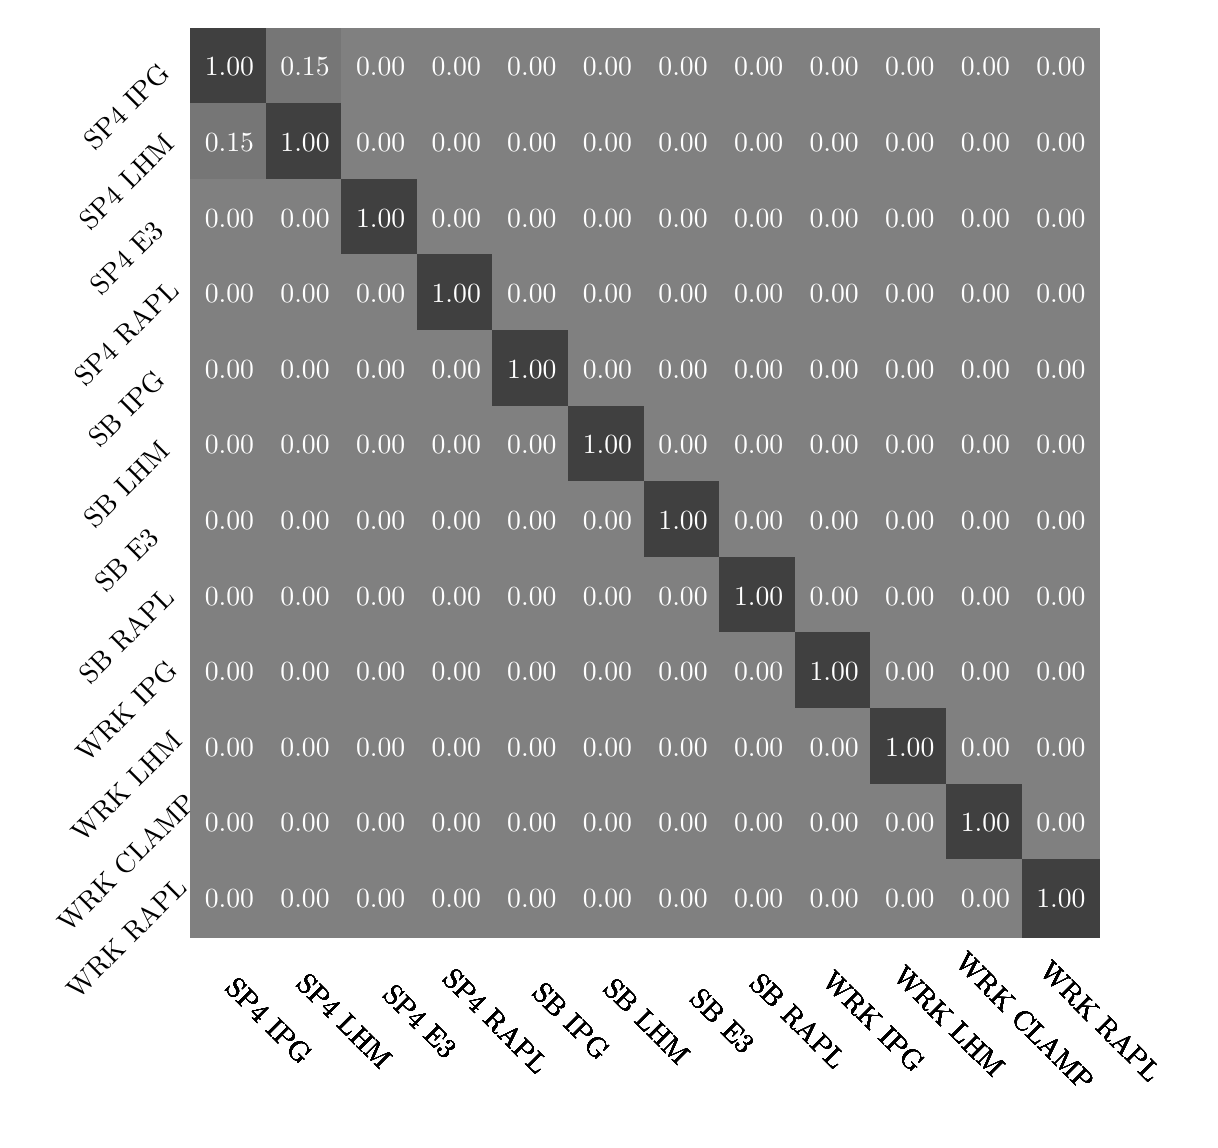
\begin{tikzpicture}[scale=0.6]
    \foreach \y [count=\n] in {{1.00, 0.15, 0.00, 0.00, 0.00, 0.00, 0.00, 0.00, 0.00, 0.00, 0.00, 0.00},{0.15, 1.00, 0.00, 0.00, 0.00, 0.00, 0.00, 0.00, 0.00, 0.00, 0.00, 0.00},{0.00, 0.00, 1.00, 0.00, 0.00, 0.00, 0.00, 0.00, 0.00, 0.00, 0.00, 0.00},{0.00, 0.00, 0.00, 1.00, 0.00, 0.00, 0.00, 0.00, 0.00, 0.00, 0.00, 0.00},{0.00, 0.00, 0.00, 0.00, 1.00, 0.00, 0.00, 0.00, 0.00, 0.00, 0.00, 0.00},{0.00, 0.00, 0.00, 0.00, 0.00, 1.00, 0.00, 0.00, 0.00, 0.00, 0.00, 0.00},{0.00, 0.00, 0.00, 0.00, 0.00, 0.00, 1.00, 0.00, 0.00, 0.00, 0.00, 0.00},{0.00, 0.00, 0.00, 0.00, 0.00, 0.00, 0.00, 1.00, 0.00, 0.00, 0.00, 0.00},{0.00, 0.00, 0.00, 0.00, 0.00, 0.00, 0.00, 0.00, 1.00, 0.00, 0.00, 0.00},{0.00, 0.00, 0.00, 0.00, 0.00, 0.00, 0.00, 0.00, 0.00, 1.00, 0.00, 0.00},{0.00, 0.00, 0.00, 0.00, 0.00, 0.00, 0.00, 0.00, 0.00, 0.00, 1.00, 0.00},{0.00, 0.00, 0.00, 0.00, 0.00, 0.00, 0.00, 0.00, 0.00, 0.00, 0.00, 1.00},} {
    % column labels
    \foreach \a [count=\n] in {SP4 IPG,SP4 LHM,SP4 E3,SP4 RAPL,SB IPG,SB LHM,SB E3,SB RAPL,WRK IPG,WRK LHM,WRK CLAMP,WRK RAPL} {
      \node[minimum size=10mm, xshift=0.5cm, rotate=-45] at (\n*1.6, -21.8) {\a};
    }
    % heatmap tiles
    \foreach \x [count=\m] in \y {
      \pgfmathsetmacro{\xa }{(\x + 1) / 2 * 100}
      \node[fill=darkgray!\xa!lightgray, minimum size=10mm, text=white, font={\normalsize}] at (\m*1.6,-\n*1.6) {\x};
    }
  }
    % row labels
    \foreach \a [count=\i] in {SP4 IPG,SP4 LHM,SP4 E3,SP4 RAPL,SB IPG,SB LHM,SB E3,SB RAPL,WRK IPG,WRK LHM,WRK CLAMP,WRK RAPL} {
      \node[minimum size=10mm, xshift=-0.35cm, yshift=-0.5cm, rotate=45] at (0,-\i*1.6) {\a};
    }
  \end{tikzpicture}
  \caption{Here the results for the FannkuchRedux can be seen}
  \label{tab:HeatFannkuchRedux}
  \end{figure} 

As can be seen in \cref{tab:HeatFannkuchRedux}, the majority of the values are below $p = 0.05$. When $p < 0.05$ the null hypothesis is rejected, which it is only with a few exceptions, including SP4 LHM and SP4 IPG. This could indicate that IPG and LHM might not be independent of each other, we have suspected from the results that the measurements from these two are done the same way. This serves as another indication of this hypothesis being true. However to further investigate this is future work.
This aligns with the expectations that the samples are mostly independent of each other in the majority of cases.

\subsection{Correlation}\label{subsec:correlation1}
In this section the correlation between the data will be calculated. To do this Kendall's Tau coefficient\cite{kendall1938new} described in \cref{subsec:NormalDist1} will be used, as the data was not normally distributed. When testing the test case measurements from experiment \#1 with Kendall's Tau coefficient, the following data is processed in the following manner. When using Kendall's Tau coefficient, the test case measurements for each of the test cases were combined for each DUT, and sorted based on the test case, where an example of this can be seen in \cref{tab:RainBowGraph}.

\input{tabels/experiment_results/exp_one/StatQuest/stats.tex}

\paragraph{Expectations:} The expectations are that all of the measuring instruments will be positively correlated with each other. The exact correlation is difficult to predict, but a positive correlation is expected. When calculating correlation higher correlations would generally be more indicative of valid measurements, as it shows the measuring instruments agreeing.

\paragraph{Result:} The correlation between DUTs and measuring instruments can be observed in \cref{tab:correlationWork},  \cref{tab:correlationSurfB} and \cref{tab:correlationSurfP} for the workstation Surface Pro 4 and Surface Book respectively.

\begin{figure}
\centering
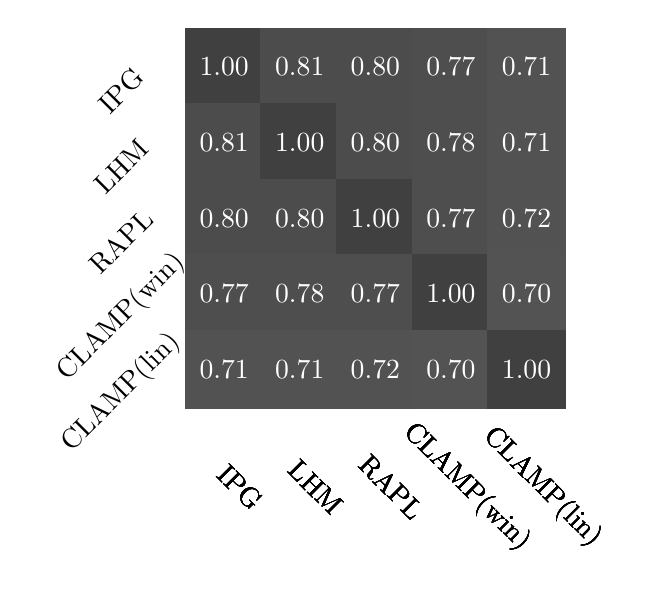
\begin{tikzpicture}[scale=0.6]
  \foreach \y [count=\n] in {{1.00, 0.81, 0.80, 0.77, 0.71},{0.81, 1.00, 0.80, 0.78, 0.71},{0.80, 0.80, 1.00, 0.77, 0.72},{0.77, 0.78, 0.77, 1.00, 0.70},{0.71, 0.71, 0.72, 0.70, 1.00},} {
  % column labels
  \foreach \a [count=\n] in {IPG,LHM,RAPL,CLAMP(win),CLAMP(lin)} {
    \node[minimum size=10mm, xshift=0.2cm, rotate=-45] at (\n*1.6, -10.50) {\a};
  }
  % heatmap tiles
  \foreach \x [count=\m] in \y {
    \pgfmathsetmacro{\xa }{(\x + 1) / 2 * 100}
    \node[fill=darkgray!\xa!lightgray, minimum size=10mm, text=white, font={\normalsize}] at (\m*1.6,-\n*1.6) {\x};
  }
}
  % row labels
  \foreach \a [count=\i] in {IPG,LHM,RAPL,CLAMP(win),CLAMP(lin)} {
    \node[minimum size=10mm, xshift=-0.35cm, yshift=-0.3cm, rotate=45] at (0,-\i*1.6) {\a};
  } 
\end{tikzpicture}
\caption{This heat map represents Correlation coefficients between the different measuring instruments -1 to 1 on the Workstation}
\label{tab:correlationWork}
\end{figure}
\begin{figure}
    \centering
    \begin{subfigure}{.5\textwidth}
      \centering
      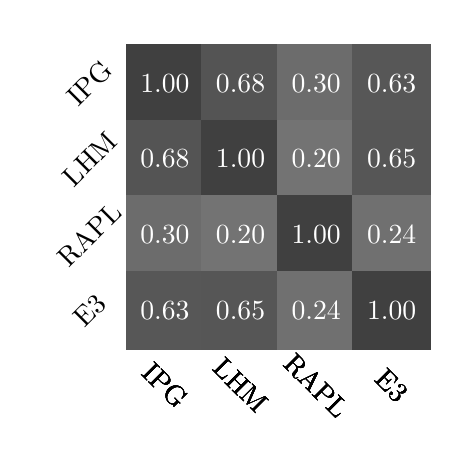
\begin{tikzpicture}[scale=0.6]
        \foreach \y [count=\n] in {{1.00, 0.68, 0.30, 0.63},{0.68, 1.00, 0.20, 0.65},{0.30, 0.20, 1.00, 0.24},{0.63, 0.65, 0.24, 1.00},} {
        % column labels
        \foreach \a [count=\n] in {IPG,LHM,RAPL,E3} {
          \node[minimum size=10mm, xshift=0.0cm, rotate=-45] at (\n*1.6, -8) {\a};
        }
        % heatmap tiles
        \foreach \x [count=\m] in \y {
          \pgfmathsetmacro{\xa }{(\x + 1) / 2 * 100}
          \node[fill=darkgray!\xa!lightgray, minimum size=10mm, text=white, font={\normalsize}] at (\m*1.6,-\n*1.6) {\x};
        }
      }
        % row labels
        \foreach \a [count=\i] in {IPG,LHM,RAPL,E3} {
          \node[minimum size=10mm, xshift=-0.0cm, yshift=-0.0cm, rotate=45] at (0,-\i*1.6) {\a};
        }
      \end{tikzpicture}
    \caption{This heat map represents Correlation coefficients between the different measurement instruments -1 to 1 on the Surface Book}
    \label{tab:correlationSurfP}
    \end{subfigure}%
    \begin{subfigure}{.5\textwidth}
      \centering
      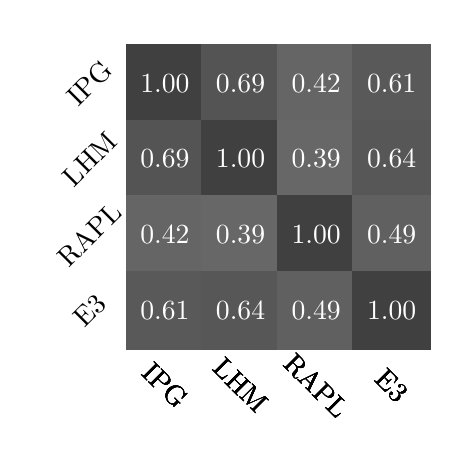
\begin{tikzpicture}[scale=0.6]
        \foreach \y [count=\n] in {{1.00, 0.69, 0.42, 0.61},{0.69, 1.00, 0.39, 0.64},{0.42, 0.39, 1.00, 0.49},{0.61, 0.64, 0.49, 1.00},} {
        % column labels
        \foreach \a [count=\n] in {IPG,LHM,RAPL,E3} {
          \node[minimum size=10mm, xshift=0.0cm, rotate=-45] at (\n*1.6, -8) {\a};
        }
        % heatmap tiles
        \foreach \x [count=\m] in \y {
          \pgfmathsetmacro{\xa }{(\x + 1) / 2 * 100}
          \node[fill=darkgray!\xa!lightgray, minimum size=10mm, text=white, font={\normalsize}] at (\m*1.6,-\n*1.6) {\x};
        }
      }
        % row labels
        \foreach \a [count=\i] in {IPG,LHM,RAPL,E3} {
          \node[minimum size=10mm, xshift=-0.0cm, yshift=-0.0cm, rotate=45] at (0,-\i*1.6) {\a};
        }
      \end{tikzpicture}
    \caption{This heat map represents Correlation coefficients between the different measurement instruments -1 to 1 on the Surface Pro 4}
    \label{tab:HeatFasta}
    \end{subfigure}
\end{figure}

These results match our expectations as all of the correlations are positive. A more in depth analysis of these results will be conducted in the following paragraphs, based on \textbf{RQ2-4}.

\paragraph{RQ2:} When comparing the measuring instrument with each other, the correlations coefficients found in \cref{subsec:correlation1} is used and when evaluating the results, the scale presented by Guildford in \cite[219]{guilford1950fundamental} is used. The values for the scale can be found in \cref{tab:GuildfordScale}.

\begin{table}[ht]
    \centering
    \begin{tabular}{|| c | c ||}
        \hline
        \textbf{Values} & \textbf{Label} \\ [0.5ex] \hline\hline
        $<.20$ & Slight; almost negligible relationship \\
        $.20-.40$ & Low correlation; definite but small relationship \\
        $.40-.70$ & Moderate correlation; substantial relationship \\
        $.70-.90$ & High Correlation; marked relationship \\
        $.90-1$ & Very high correlation; very dependable relationship \\ \hline
    \end{tabular}
    \caption{The values for the scale presented by Guildford in \cite[219]{guilford1950fundamental}}\label{tab:GuildfordScale}
\end{table}

Using this scale we evaluate the correlation between the different measuring instruments. Looking across the different DUTs we calculate the average correlation between each of the measuring instruments. This can only be done for the measuring instruments IPG, LHM and RAPL, as these are the only measuring instruments used on all DUTs. When comparing the correlation between the different measuring instruments across all DUTs, the average correlation is as follows:

$$IPG | LHM = (0.68+0.81+0.69)/3 = 0.726$$
$$IPG | RAPL = (0.30+0.42+0.80)/3 = 0.506$$
$$LHM | RAPL = (0.80+0.39+0.21)/3 = 0.466$$

Next up, the average correlation between the different software measuring instruments against the clamp is calculated. This is done for only the workstation, as the clamp was only used on this DUT.

$$IPG | Clamp = (0.77+0.71)/2 = 0.74$$
$$LHM | Clamp = (0.78+0.71)/2 = 0.745$$
$$RAPL | Clamp = (0.77+0.72)/2 = 0.745$$

Similarly, the average correlation between the different measuring instruments from the DUTs with a battery is calculated, to see how they are correlated with E3.

$$IPG | E3 = (0.63+0.61)/2 = 0.62$$
$$LHM | E3 = (0.65+0.64)/2 = 0.645$$
$$RAPL | E3 = (0.24+0.49)/2 = 0.365$$

Looking at these numbers and evaluating them on the Guildford scale, we see that IPG | LHM, IPG | Clamp and RAPL | Clamp all are highly correlated, while LHM | RAPL, LHM | RAPL, IPG | E3 and LHM | E3 has substantial relationships. The lowest correlation between the measurements was found with RAPL | E3 which is a low correlation.

\paragraph{RQ3:} In regards to the different OSs and how these affect the results, it can be seen that there are differences between the measurements conducted on Linux and Windows. When looking at the coefficients for RAPL and the clamp on Linux, it can be observed that they are generally less correlated with the other measuring instruments on Windows. This can be seen when calculating the average coefficients for each of the instruments across the different DUTs.

\begin{itemize}
    \item \textbf{Windows}
    \begin{itemize}
        \item IPG: $0.642$ %0.81+0.80+0.77+0.71+0.68+0.30+0.63+0.69+0.42+0.61
        \item LHM: $0.635$ %0.81+0.8+0.78+0.71+0.68+0.2+0.65+0.69+0.39+0.64
        \item Clamp: $0.755$ %0.77+0.78+0.77+0.70
        \item E3: $0.543$ %0.63+0.65+0.61+0.64+0.24+0.49
    \end{itemize}
    \item \textbf{Linux}
    \begin{itemize}
        \item Clamp: $0.71$ %0.71+0.71+0.72+0.70
        \item RAPL: $0.513$ %0.80+0.80+0.77+0.72+0.3+0.2+0.24+0.42+0.39+0.49
    \end{itemize}
\end{itemize}

Looking at these numbers it can be seen that RAPL and the hardware measurements on Linux are generally less correlated with the rest of the measuring instruments. This does make sense as they are different OSs and would be expected to have different power consumption.

\paragraph{RQ4}: Similarly comparing the different DUTs it is found that there are significant differences in how correlated the measuring instruments are on each DUT.

\begin{itemize}
    \item \textbf{Workstation}
    \begin{itemize}
        \item IPG, LHM, Clamp, RAPL: $0.757$%
    \end{itemize}
    \item \textbf{Surface 4 Pro}
    \begin{itemize}
        \item IPG, LHM, E3, RAP: $0.540$%0.69+0.42+0.61+0.39+0.64+0.49
    \end{itemize}
    \item \textbf{Surface Book}
    \begin{itemize}
        \item IPG, LHM, E3, RAP: $0.450$ %0.68+0.30+0.63+0.20+0.65+0.24
    \end{itemize}
\end{itemize}

When comparing the different DUTs it can be observed that the measuring instruments are more correlated with each other on the Workstation than on the two laptops. When comparing the two laptops it can be seen that the Surface Book has significantly lower coefficients than the Surface 4 Pro. Looking closely at the numbers they are very similar in all cases except for RAPL, where the Surface Book performance is worse.

\begin{itemize}
    \item \textbf{Surface Book}
    \begin{itemize}
        \item RAPL: $0.246$
    \end{itemize}
    \item \textbf{Surface Pro 4}
    \begin{itemize}
        \item RAPL: $0.433$
    \end{itemize}
\end{itemize}
% $$$$ 
% % \begin{figure}
    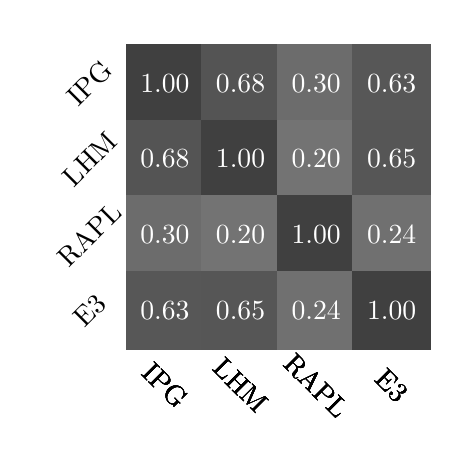
\begin{tikzpicture}[scale=0.6]
        \foreach \y [count=\n] in {{1.00, 0.68, 0.30, 0.63},{0.68, 1.00, 0.20, 0.65},{0.30, 0.20, 1.00, 0.24},{0.63, 0.65, 0.24, 1.00},} {
        % column labels
        \foreach \a [count=\n] in {IPG,LHM,RAPL,E3} {
          \node[minimum size=10mm, xshift=0.0cm, rotate=-45] at (\n*1.6, -8) {\a};
        }
        % heatmap tiles
        \foreach \x [count=\m] in \y {
          \pgfmathsetmacro{\xa }{(\x + 1) / 2 * 100}
          \node[fill=darkgray!\xa!lightgray, minimum size=10mm, text=white, font={\normalsize}] at (\m*1.6,-\n*1.6) {\x};
        }
      }
        % row labels
        \foreach \a [count=\i] in {IPG,LHM,RAPL,E3} {
          \node[minimum size=10mm, xshift=-0.0cm, yshift=-0.0cm, rotate=45] at (0,-\i*1.6) {\a};
        }
      \end{tikzpicture}
    \caption{This heat map represents Correlation coefficients between the different measurement instruments -1 to 1 on the Surface Book}
    \label{tab:correlationSurfP}
\end{figure}
% % \begin{figure}
    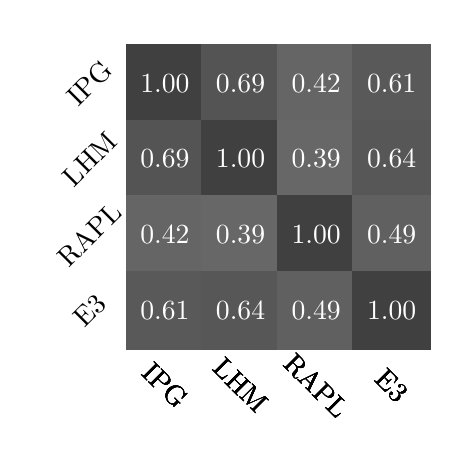
\begin{tikzpicture}[scale=0.6]
        \foreach \y [count=\n] in {{1.00, 0.69, 0.42, 0.61},{0.69, 1.00, 0.39, 0.64},{0.42, 0.39, 1.00, 0.49},{0.61, 0.64, 0.49, 1.00},} {
        % column labels
        \foreach \a [count=\n] in {IPG,LHM,RAPL,E3} {
          \node[minimum size=10mm, xshift=0.0cm, rotate=-45] at (\n*1.6, -8) {\a};
        }
        % heatmap tiles
        \foreach \x [count=\m] in \y {
          \pgfmathsetmacro{\xa }{(\x + 1) / 2 * 100}
          \node[fill=darkgray!\xa!lightgray, minimum size=10mm, text=white, font={\normalsize}] at (\m*1.6,-\n*1.6) {\x};
        }
      }
        % row labels
        \foreach \a [count=\i] in {IPG,LHM,RAPL,E3} {
          \node[minimum size=10mm, xshift=-0.0cm, yshift=-0.0cm, rotate=45] at (0,-\i*1.6) {\a};
        }
      \end{tikzpicture}
    \caption{This heat map represents Correlation coefficients between the different measuring instrument1 on the Surface Pro 4}
    \label{tab:HeatFasta}
\end{figure}





% These results seem to indicate that all of the measuring instruments are correlated, which is expected as they measure the energy consumption of the same test cases, on the same DUT's. Another interesting thing to note here is that the correlation between the measurements on the workstation are higher as opposed to the two laptops as can be seen on \cref{tab:correlationWork,tab:CobineddCorrelation}. From this it can be seen that most of the measuring instruments are at least moderate correlated, except RAPL | E3.

%and this is especially true when looking at the workstation. %Another interesting observation is that all the measurements are less correlated on the laptops than the Workstation.




